% -----------------------------------------------
% Template for ISMIR Papers
% 2015 version, based on previous ISMIR templates
% -----------------------------------------------

\documentclass{article}
\usepackage{ismir,amsmath,cite}
\usepackage{graphicx}
\usepackage{color}
\usepackage{amsfonts}
\usepackage{brian}
\usepackage{qtree}
\usepackage{caption}
\usepackage{subcaption}
% \def\shag{\ensuremath{\text{\textsc{SHAG}}}}
%\def\shag{\ensuremath{\mathpzc{H}}}
\def\shag{\ensuremath{\mathpzc{T}}}
\DeclareMathAlphabet{\mathpzc}{OT1}{pzc}{m}{it}

% Title.
% ------
\title{Hierarchical Evaluation of Segment Boundary Detection}

% Single address
% To use with only one author or several with the same address
% ---------------
%\oneauthor
% {Names should be omitted for double-blind reviewing}
% {Affiliations should be omitted for double-blind reviewing}

% Two addresses
% --------------
\twoauthors
  {First author} {School \\ Department}
  {Second author} {Company \\ Address}

% Three addresses
% --------------
%\threeauthors
  %{First author} {Affiliation1 \\ {\tt author1@ismir.edu}}
  %{Second author} {\bf Retain these fake authors in\\\bf submission to preserve the formatting}
  %{Third author} {Affiliation3 \\ {\tt author3@ismir.edu}}

% Four addresses
% --------------
%\fourauthors
%  {First author} {Affiliation1 \\ {\tt author1@ismir.edu}}
%  {Second author}{Affiliation2 \\ {\tt author2@ismir.edu}}
%  {Third author} {Affiliation3 \\ {\tt author3@ismir.edu}}
%  {Fourth author} {Affiliation4 \\ {\tt author4@ismir.edu}}

\begin{document}
%
\maketitle
%
\begin{abstract}
Structure in music is traditionally analyzed hierarchically: large-scale sections can be sub-divided and refined down to the short melodic ideas at the motivic level. 
However, typical algorithmic approaches to structural annotation produce flat temporal partitions of a track, which are commonly evaluated against a similarly flat, human-produced
annotation. Evaluating structure analysis as represented by flat annotations effectively discards all notions of structural depth in the evaluation.
Although collections of hierarchical structure annotations have been recently published, no techniques yet exist to measure an algorithm's accuracy against these rich structural annotations.
In this work, we propose a method to evaluate structural boundary detection with hierarchical annotations.
The proposed method transforms boundary detection into a ranking problem, and facilitates the comparison of
both flat and hierarchical annotations.
We demonstrate the behavior of the proposed method with various synthetic and real
examples drawn from the SALAMI dataset. 
\end{abstract}
%
\section{Introduction}\label{sec:introduction}

The analysis of structure in music has been a principal area of interest by musicologists for many years.
Its goal is to identify and categorize the form of a musical piece by investigating the organization of its components, such as sections, phrases, melodies, or recurring motives.
Traditional analyses usually provide multiple levels of annotation (\eg, Schenkerian analysis), which reinforce the general assumption that music is structured hierarchically~\cite{Lerdahl1983a}.
Consequently, tree representations are commonly used to both model and analyze hierarchical forms in music~\cite{Lerdahl1983}.

In the music information research literature, \emph{music segmentation} (also known as \emph{music structure
analysis}) is a task that aims to automatically identify the structure of a musical recording~\cite{Paulus2010}.
The segmentation task has historically been geared toward algorithms which analyze a recording and produce a
flat partition of time segments.
This formalization contrasts with our intuition that music exhibits hierarchical
structure~\cite{Peeters2009}.
Even though a large dataset of hierarchically-structured human annotations is now publicly
available~\cite{Smith2011},
% Still, most existing algorithms only operate at a flat level, likely because (i) this task is already challenging at this level~\cite{Skywalker2014}, and (ii) even if an algorithm could 
% estimate hierarchical segments, no method to evaluate them has been proposed.
current evaluation methodologies are defined only for \emph{flat} segmentations.
As a result, the dimension of \emph{depth} has been practically ignored in the evaluation of music segmentation algorithms.

In contrast to segmentation, the \emph{pattern discovery} task formulation allows output segments to overlap, 
and the output is not required to cover the entire piece.
These two tasks share multiple attributes~\cite{Nieto2014_Motives}, and steps toward a 
general formulation musical structure analysis could be made by accounting for depth in segmentation.
Numerous metrics to evaluate pattern discovery have been proposed~\cite{Collins2013}.
However, they are designed to capture repeated patterns, and would be inappropriate for 
evaluating non-repeating, hierarchical structure.

%This automatic task could facilitate, e.g., the intra-piece navigation, generation of music summaries, or segment-based recommendation systems, especially nowadays when listeners have easy access to large digital music collections.
%Nevertheless, the vast majority of music segmentation algorithms only operate at a flat level instead of following the hierarchical approach that most musicologists follow.

\subsection{Our contributions}
We present the \emph{Tree Measures} ($T$-measures): an evaluation framework designed
to measure the accuracy of boundary detection in hierarchical segmentations.
%The proposed metrics work at a frame-level --- similar to the method proposed by Levy and Sandler to evaluate structural annotations~\cite{Levy2008} --- and they are based on a rank retrieval evaluation where each frame is ranked depending on whether it belongs to the \emph{correct} segment.
The $T$-measures operate by inferring frame-wise similarity from a hierarchical annotation, and then comparing 
the induced rank-orderings of frames to assess agreement between reference and estimated annotations.
The $T$-measures integrate information from all layers of a hierarchy, but also trivially
specialize to handle flat annotations, and require no explicit correspondence between the
depth of the estimated and reference hierarchies.
The $T$-measures seamlessly thus encourage the development of new algorithms to produce richer representations of structure.
We demonstrate the behavior of the $T$-measures with multiple synthetic and human examples, and compare the scores with existing methods when possible.

%The rest of the paper is organized as follows:
%In \Cref{sec:curr_meth} we review the current evaluation methods of (flat) boundary algorithms. 
%The proposed metric is formally introduced in \Cref{sec:eval_desc}. 
%We provide multiple examples to illustrate the behavior of the $T$-measures in \Cref{sec:examples}.
%Finally, we draw conclusions and discuss future work in \Cref{sec:conclusions}.

\section{Segment Boundary Evaluation}\label{sec:curr_meth}

Segmentation algorithms are typically evaluated for two distinct goals.  
The first goal, \emph{boundary detection}, evaluates the algorithm's ability to detect the times of transitions between segments.
The second goal, \emph{structural grouping}, evaluates the labeling applied to the estimated segmentation, and thus quantifies the ability of an algorithm to detect repeated forms, such as verses or refrains. 
In this paper, we focus exclusively on the boundary detection task.

Boundary estimates are typically evaluated by precision and recall~\cite{turnbull2007supervised}.
Estimated and reference boundaries are matched within a specified tolerance window --- typically either 0.5 or 3 seconds --- and the hit rate $n_h$ (number of matches) is used to define precision and recall scores:
\begin{equation}
P \defeq \frac{n_h}{n_e}, \quad\quad R \defeq \frac{n_h}{n_r},
\end{equation}
where $n_e$ and $n_r$ denote the number of boundaries in the estimated and reference
annotations, respectively.
$P$ and $R$ are typically combined into a single $F$-measure by computing their harmonic mean.

Boundary detection has also been evaluated by \emph{deviation}~\cite{turnbull2007supervised}.
This is done by measuring the median time (absolute) differential between each reference boundary and the nearest estimated boundary (\emph{R2E}), and vice versa (\emph{E2R}).
Boundary deviation is useful for quantifying the temporal accuracy of a detection event.
However, it can be sensitive to the number of estimated boundaries.

\subsection{The limitations of flat evaluation}
The precision-recall paradigm has been critical to quantifying improvements in segmentation algorithms, but it has numerous limitations with hierarchical annotations.
The most obvious limitation is that both the reference and estimated annotations must have flat structure.
This is sometimes resolved by collecting multiple flat reference annotations for each track, 
each corresponding to a different level of analysis~\cite{Smith2011}.

When only the estimation is flat, it is still not obvious how to compute accuracy against multiple layers.
Na\"ive aggregation of reference boundaries across all layers prior to evaluation would imply 
that all boundaries are equally informative.
Hierarchical constraints imply that boundaries at low levels outnumber those at high levels.
However, high-level boundaries often convey more information about the overall structure of the piece, but
their contribution to the total score may be diluted by the abundance of low-level boundaries.

On the other hand, flat scoring before aggregation across layers can be problematic as well, 
since it discards the relational structure between layers in the reference annotation.
This can complicate interpretation of the scores by conflating inaccurate boundary detection
with mismatch between the target levels of the estimate and reference annotations~\cite{Smith2013}.

Finally, the above strategies provide no means to directly compare two hierarchical annotations.
While one may imagine simple comparison strategies when both hierarchies have a small
number of layers with an obvious layer-wise correspondence 
--- \eg, SALAMI's \emph{large}- and \emph{small}-scale annotations --- it may not be clear how to proceed in
more general settings.
% Talk about how good performance at one vs. the other leads to difficult interpretation, eg 0.5 vs. 3s in smith 2014

%As an example, \Cref{trees} depicts two distinct structural decompositions of a song $S$, first into high-level components $A$ and $B$, and then into small components $a, b, c$.
%While both trees produce the same set of boundaries at the bottom layer, the structural interpretation is significantly different.
%This hierarchical information would be lost by any form of independent, layer-wise evaluation.

%\begin{figure}
%  \centering
%  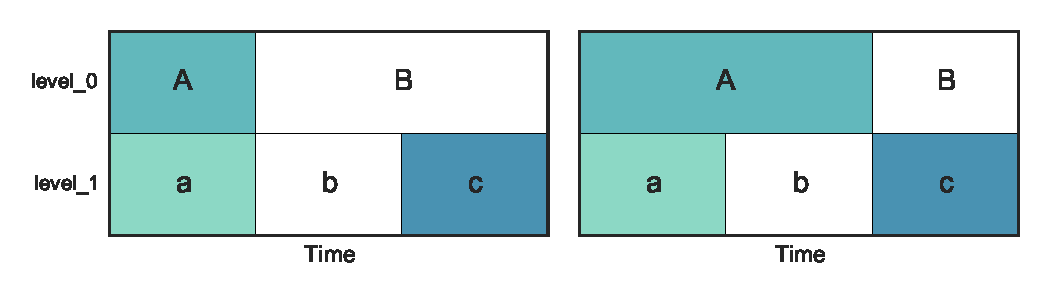
\includegraphics[width=0.45\textwidth]{figs/toy-examples.pdf}
%\caption{A toy example of two hierarchical annotation structures with identical flattened segmentations, but distinct structural interpretations.\label{trees}}
%\end{figure}

\section{The Tree Measures}\label{sec:eval_desc}
\sloppy
In this section, we derive the \emph{tree measures} for evaluating multi-level structural boundary detection.
%The proposed evaluation scheme explicitly accounts for cross-layer structure in segmentation, and directly accommodates multiple layers of specificity in both the reference and estimation.
The evaluation is based on a reduction to ranking evaluation, which we describe in detail below.

\subsection{Preliminaries}

% Let denote a song as represented by a time series of 
% feature data, where $d$ denotes the dimension of features, and $n$ denotes the
% time duration at some fixed resolution $f_r$ (\eg, 10Hz).
% Flat segmentation evaluation schemes suppose a single partitioning into $m$
% temporally contiguous regions, so that $X=[X_1|X_2|\cdots|X_m]$.  
% Instead, we will allow for a hierarchical decomposition

Let $X$ denote a set of sample frames generated from the track at some fixed resolution $f_r$ (\eg,
10Hz).\footnote{Non-uniform samplings (\eg, beat- or onset-aligned samples) are also easily accommodated.}
Let $S $ denote a flat, temporally contiguous partition of $X$,
and let $S(i)$ identify the segment containing the $i$th frame in $X$.
We will use the subscripts $S_R$ and $S_E$ to denote \emph{reference} and \emph{estimated} annotations, respectively.

A \emph{hierarchical segmentation} $H$ is defined as a sequence of flat segmentations $(S^0, S^1, \dots, S^d)$ where each layer is a \emph{refinement}
of the preceding layer.\footnote{A partition $S^{i+1}$ is a refinement of partition $S^{i}$ if each member of $S^{i+1}$ is contained within exactly one member of $S^i$.}
Let $H(i,j)$ identify the smallest (most refined) segment containing frames $i$ and $j$.
We will denote precedence (containment) of segments by $\prec$: \eg, $H(j, k) \prec H(i, k)$.
Note that flat segmentations are a special case of hierarchical segmentations, where there are only two
levels of segmentation, and the first layer contains no boundaries.

As illustrated in \Cref{fig:hier-example}, hierarchical segmentations can be represented as tree structures.
%\footnote{To simplify illustrations, the top-level segment spanning the entire track is suppressed.}
Here, $H(i, i), H(j, j)$ and $H(k,k)$ denote the most specific segments containing frame $i, j$ and $k$,
respectively.
From the figure, we observe that $H(j,k)$ identifies the least common ancestor of frames $j$ and $k$.
We can generally infer membership and precedence relations from the hierarchy, \eg,
\begin{equation}
j \in H(j, j) \prec H(j, k) \prec H(i, j) = H(i, k).
\end{equation}


\begin{figure}
  \centering
  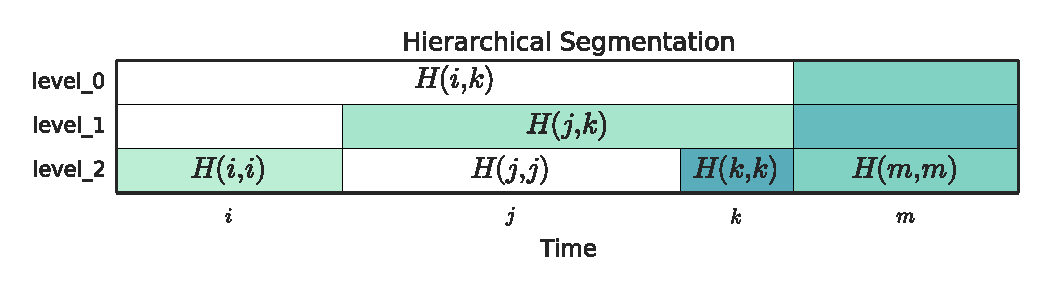
\includegraphics[width=\columnwidth]{figs/hier-example.pdf}
  \caption{An example of a three-level hierarchical segmentation.
  Example frames $i, j,$ and $k$ are indicated along the $x$-axis, and their containing segments are indicated
  within the figure, \eg, $H(j, k)$.}
  \label{fig:hier-example}
\end{figure}


\subsection{Flat segmentation and bipartite ranking}

Segmentation evaluation can be reduced to a ranking evaluation problem as follows.
Let $q$ denote an arbitrary frame, and let $i$ and $j$ denote any two frames such that $S_R(q) = S_R(i)$ and $S_R(q) \neq S_R(j)$.
In this case, $i$ may be considered \emph{relevant} for $q$, and $j$ is considered \emph{irrelevant}.
This leads to the following per-frame recall metric:
\begin{align}
f(q ; S_E, S_R) &\defeq  \hspace{-1.5em} \sum_{\substack{i \in S_R(q) \setminus \{q\},\\ j \notin S_R(q)}}
\hspace{-1.5em}\frac{\ind{S_E(q) = S_E(i) \neq S_E(j) }}{Z_q} \label{flatrecall}\\
Z_q &\defeq (|S_R(q)| - 1)\cdot (n - |S_R(q)| + 1), \notag
\end{align}
where $\ind{\cdot}$ is the indicator function, $n = |X|$ denotes the total number of frames, and $Z_q$
counts the number of terms in the summation.
The score for frame $q$ is the fraction of pairs $(i, j)$ for which $S_E$
agrees with $S_R$ with respect to $q$.
Averaging over all $q$ yields a mean recall score:
\begin{equation}
\rho(S_E, S_R) \defeq \frac{1}{n} \sum_q f(q ; S_E, S_R).\label{avgrecall}
\end{equation}


\subsection{Hierarchies and partial ranking}

\Cref{flatrecall} is defined in terms of segment membership (in)equalities, but it has a straightforward 
generalized to hierarchical segmentations.
If we restrict attention to a query sample $q$, then $H(q, \cdot)$ induces a partial ranking over the remaining samples.
Frames contained in $H(q, q)$ are considered maximally relevant, followed by those in $H(q, q)$'s immediate ancestor, and so on.

Rather than compare frames $q$, $i$, and $j$ where ${S(q) = S(i) \neq S(j)}$, we can instead compare where
$H(q, i) \prec H(q, j)$: \ie, the pair $(q,i)$ merge deeper in the hierarchy than do $(q,j)$.
This leads to the following generalization of \Cref{flatrecall}:
\begin{equation}
    g(q ; H_E, H_R) \defeq \hspace{-1.5em} \sum_{\substack{(i, j),\\ i \neq q,\\ H_R(q, i) \prec H_R(q, j)}}
    \hspace{-1.5em} \frac{\ind{H_E(q, i) \prec H_E(q, j)}}{Z_q}.\label{hierrecall}
\end{equation}
where $Z_q$ is suitably modified to count the number of terms in the summation.
This definition is equivalent to \Cref{flatrecall} for flat hierarchies, but it applies more generally to 
hierarchies of arbitrary (and unequal) depth.

Just as in \Cref{flatrecall}, $g$ can be viewed as a classification accuracy of correctly predicting pairs $(i, j)$ as positive ($q$ and $i$ merge first) or negative ($q$ and $j$ merge first).
Ties ($H(q, i) = H(q, j)$) are precluded by the strict precedence operator in the summation.
\Cref{hierrecall} can be alternately be viewed as a generalized area under the curve (AUC) over the partial
ranking induced by the hierarchical segmentation, where depth within the estimated hierarchy $H_E$ plays the
role of the detection threshold.

% Note that the precedence comparisons here are strict, so we never compare two $i$ and $j$ that merge simultaneously with $q$.
Averaging over $q$ yields the \emph{tree-recall} $T$-measure:
\begin{equation}
\shag_R(H_E, H_R) \defeq \frac{1}{n} \sum_q g(q ; H_E, H_R).\label{shagunder}
\end{equation}
The \emph{tree-precision} metric $\shag_P(H_E)$ is defined analogously by swapping the roles of $H_E$ and $H_R$:
\begin{equation}
\shag_P(H_E, H_R) \defeq \shag_R(H_R, H_E).
\end{equation}
Intuitively, $\shag_R$ measures how many triplets generated by the reference $H_R$ can be found in the estimate $H_E$, 
while $\shag_P$ computes the converse.  The $T$-measures retain interpretability as recall and precision scores,
albeit at the level of frame triplets rather than boundaries.  Finally, an analogous $F$-measure $\shag_F$ can 
be defined in the usual way by computing the harmonic mean of $\shag_P$ and $\shag_R$.

% Note this loss is equivalent to that evaluated by for subjective artist similarity~\cite{mcfee2011}.
% The difference here is that the reference rankings are induced from ordinal data, and not subject to consistency errors.

\subsection{Windowing in Time}
\label{sec:window}

The $T$-measures defined above capture the basic notion of hierarchically nested, frame-level relevance, but
they pose three technical limitations.
First, the score for each query will generally depend on the track duration $n$, which makes comparisons between tracks of differing length problematic.  
Second, for large values of $n$ (long tracks), \Cref{hierrecall} can be dominated by trivially irrelevant comparison points $j$ which lie far from $q$ in time, \ie, $|q-i| \ll |q-j|$.
Longer tracks will result in relatively inflated scores when compared to shorter tracks, simply by virtue of having a large number of ``easy'' comparisons.
Finally, the calculation of the $T$-measures as defined in \Cref{shagunder} can be expensive, taking
$\Oh(n^3)$ time using a direct implementation.

To resolve these issues, we introduce a time window of $w$ seconds to both simplify the 
calculation of the metric and normalize its range.  This is achieved by
restricting the triples $(q,i,j)$ in the summation such that $i$ and $j$ both lie within
a window of $w$ seconds centered at $q$.
Adding this windowing property to equations (\ref{hierrecall},~\ref{shagunder}) yields the windowed $T$-measures:
\begin{equation}
    g(q ; H_E, H_R, w) \defeq \hspace{-1.5em} \sum_{\substack{
        i, j \in \{x : |q-x| \leq w/2\}\\ 
  i \neq q,\\
  H_R(q, i) \prec H_R(q, j) }}
  \hspace{-2em} \frac{\ind{H_E(q, i) \prec H_E(q,
  j)}}{Z_q(w)},\label{windowrecall}
\end{equation}
\begin{equation}
\shag_R(H_E, H_R ; w) \defeq \frac{1}{n} \sum_q g(q ; H_E, H_R, w),
\end{equation}
and $Z_q(w)$ is again modified to count the terms in the summation.
This reduces computational complexity from $O(n^3)$ to $\Oh(nw^2)$.
Moreover, each query frame $q$ now operates over a fixed maximum number of comparisons
$(i, j)$, and the windowed $T$-measures are comparable between tracks of different lengths (\eg, when
compiling score statistics over a collection).


\subsection{Transitive reduction}
\label{sec:transitive}

Just as \Cref{hierrecall} can be dominated by long-range interactions in the absence of windowing, deep hierarchies can also pose a problem.
To see this, consider the sequence $H_R(q, i) \prec H_R(q, j) \prec H_R(q, k)$.
Since the summation in \Cref{hierrecall} ranges over all precedence comparisons, and $i \in H_R(q, j)$, the
triple $(q, i, k)$ is double-counted.
Since segments grow in size at higher levels in the hierarchy, over-counting can dominate the evaluation.

To counteract this effect, the summation can be restricted to direct precedence relations.
In practice, this is accomplished by comparing samples only from successive levels in the hierarchy, \ie, 
replacing the partial ranking generated by $q$ with its transitive reduction.
This both eliminates redundant comparisons and increases $g$'s effective range.
We refer to the resulting metrics as \emph{reduced} $T$-measures.


%\subsection{Choosing a time window}
%Small windows (\eg, $w \leq 3$) generally capture local changes, since large-scale structural changes are not typically confined to small time intervals~\cite{Smith2013}.
%Ideally, the window should be long enough to capture boundaries of segments at multiple resolutions, but not so large as to become dominated by trivial comparisons.
%While there may not be a single window length that satisfies this criteria for all songs, we consider two practical approaches to window selection.

%First, an appropriate window length can be estimated by examining the segment duration statistics of the reference annotations.  
%For example, one may take the average duration of high-level segment annotations, as they can be expected to contain multiple small segments, and thus capture local structure.
%Second, one may report results for a multiple window parameters, as is currently done for boundary detection as described in \Cref{sec:curr_meth}.  

% Ideally, the window should be long enough to capture the boundaries of the current segments, and that is the same for all tracks in order to be able to easily compare results within a reasonable range.



\section{Examples}\label{sec:examples}

In this section we discuss the behavior of the $T$-measures by showing various synthetic examples, and compare them against other existing methods when possible.
%We show the two grades of $T$-measures (undersegmentation, oversegmentation) for all the examples in this sections
%Two different versions of each metric are used to evaluate these examples: Estimated against Reference boundaries (E2R), and the Reference boundaries against the Estimated ones (R2E).
%These results will help us illustrate the variation of the scores when swapping the references with the estimations, which, in the case of $T$-measures, has a significant impact.
For each example in this section, we illustrate the behavior of our proposed metric under different window times $w$.
This section is subdivided by type of annotations under consideration.

\subsection{Flat vs.\ flat annotations}

We first compare two flat boundary annotations to demonstrate how the $T$-measures behave compared to the standard hit rate measure at 3 seconds, as well as boundary deviation scores.
The synthesized flat boundaries are displayed on the top of \Cref{fig:flat-flat}, and they aim to capture a situation where an algorithm only estimates --- without any time deviations --- a subset of all the reference boundaries.

The hit rate scores obtain recall of 40\% and precision of 100\%, since all estimated boundaries are also in the reference, but only two out of five boundaries were retrieved.\footnote{The first and last boundaries ($0$ and $60$s) mark the beginning and end of the track, and since they 
are constant across all estimates, we suppress them during evaluation to avoid score inflation.}
The median deviations (not shown) are always 0 since we did not add any fluctuation in
the boundaries.

\begin{figure}
  \centering
  \begin{subfigure}{0.5\textwidth}
    \centering
    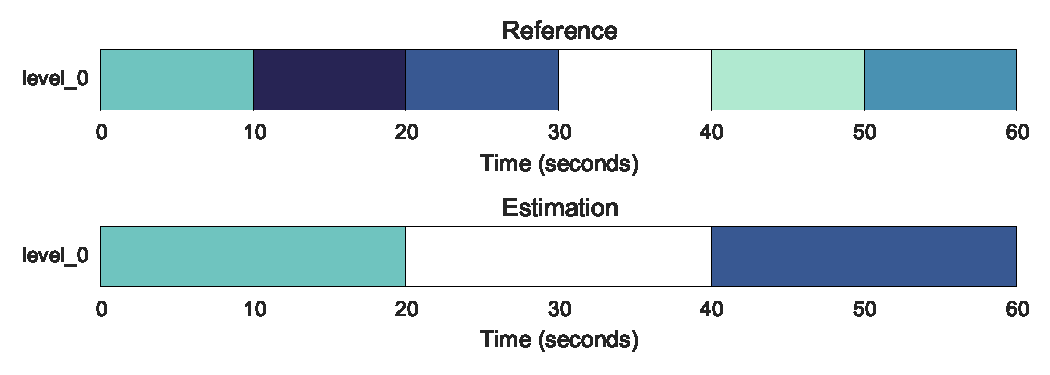
\includegraphics[width=0.94\textwidth]{figs/flat-flat.pdf}
  \end{subfigure}%
  \\
  \begin{minipage}{0.5\textwidth}
    \small
    \centering
    \vspace{10pt}
    \begin{tabular}{l|rr|rr}
      & \multicolumn{2}{c|}{\textbf{$T$-measures}} & \multicolumn{2}{c}{\textbf{Hit Rate}} \\
      $w$ & $\shag_R$   & $\shag_P$ &  $R$     & $P$ \\
      \hline
      0.5       & 0.40   & 1.00   & 0.40 & 1.00 \\
      3         & 0.40   & 1.00   & 0.40 & 1.00 \\
      15        & 0.39  & 0.53 \\
      30        & 0.69  & 0.50 \\
      $\infty$  & 0.80   & 0.50 
    \end{tabular}
  \end{minipage}
  \caption{Flat vs.\ flat boundaries (top), $T$-measures and boundary detection
    (hit-rate) scores (bottom).}
  \label{fig:flat-flat}
\end{figure}

When $w$ does not exceed the minimum segment duration, the $T$-measures coincide
with the boundary detection metrics.
For larger $w$, we observe that $\shag_P$ decreases, while $\shag_R$ increases.

To understand the relationship between $\shag_P$ and $w$, consider the example 
$(q,i,j) = (5,15,25)$.
The estimation considers $i$ to be relevant for $q$ (since they belong to the same large
segment), and $j$ to be irrelevant for $q$. Meanwhile, the reference considers both $i$
and $j$ to be equally irrelevant for $q$, so this triple contributes 0 to the precision
metric.
Note that this situation arises only when $w$ is large enough to span multiple short
segments.

In general, sensitivity to long-range interactions increases with $w$.
This illustrates how the window size must depend on the duration and scale of structure
that the practitioner wishes to capture.

\subsection{Flat vs.\ hierarchical annotations}

Here we present four different examples of flat estimations against a fixed hierarchical reference.

\subsubsection{Large-scale and over-segmentation}
\label{sec:largeover}

\Cref{fig:hier-flatlarge} illustrates a flat estimation corresponding to the highest layer of the hierarchical reference.
We report $T$-measures with and without the transitive reduction strategy described in
\Cref{sec:transitive}.  The $T$-measures behave as expected: the tree-precision score
$\shag_P$ is always 100\%, since the reference annotation agrees with the estimation at
the high level.  We also observe the general trend that \emph{full} scores exceed 
\emph{reduced} scores.

For small time windows ($w \leq 3$), the full tree-recall score is 40\%, since it
resembles the situation of \Cref{fig:flat-flat}.
The \emph{reduced} recall scores in this case are 0 because no frame $q$ in the
estimation has two frames $i, j$ both within $w \leq 3$ seconds that merge within one layer of each-other in the reference. 


\Cref{fig:hier-flatlarger} illustrates an example of a pure under-segmentation: the estimation misses a high-level structural change at 20s.  
Again, small $w$ yields $T$-measures which coincide with standard boundary detection metrics.
Larger $w$ increases the tree-recall (and decreases precision)
since only long-range interactions are well represented in the estimation.


\begin{figure}
  \centering
  \begin{subfigure}{0.5\textwidth}
    \centering
    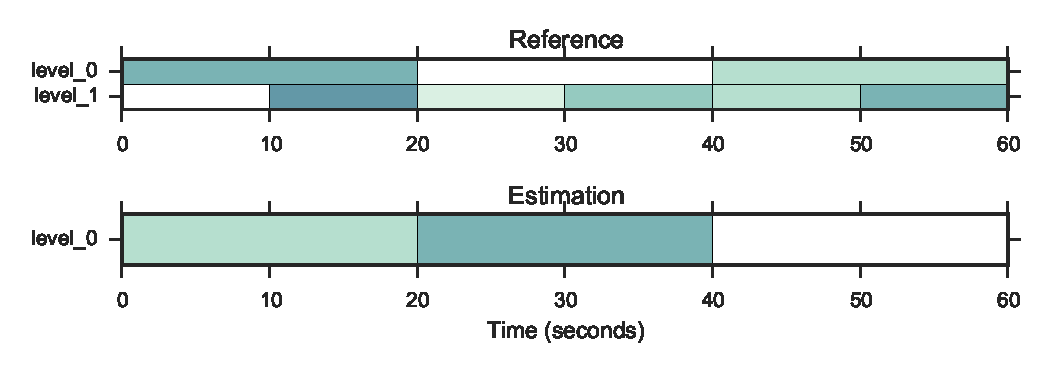
\includegraphics[width=0.94\textwidth]{figs/hier-flatlarge.pdf}
  \end{subfigure}%
  \\
  \begin{minipage}{0.5\textwidth}
    \small
    \centering
    \vspace{10pt}
    \begin{tabular}{l|rr|rr}
      & \multicolumn{2}{c|}{\textbf{Reduced}} & \multicolumn{2}{c}{\textbf{Full}} \\
      $w$       & $\shag_R$    & $\shag_P$  & $\shag_R$ & $\shag_P$    \\
      \hline
      0.5       & 0.00     & 1.00      & 0.40 & 1.00\\     
      3         & 0.00     & 1.00      & 0.40 & 1.00 \\
      15        & 0.37     & 1.00     & 0.51 & 1.00 \\
      30        & 0.70     & 1.00     & 0.82 & 1.00 \\
      $\infty$  & 0.80     & 1.00            & 0.89 & 1.00
    \end{tabular}
  \end{minipage}
  \caption{Hierarchical reference vs.\ flat (large-scale) estimation (top) and $T$-measures (bottom).  \emph{Reduced} uses the transitive reduction method of \cref{sec:transitive}, while \emph{Full} uses comparisons across all layers.}
  \label{fig:hier-flatlarge}
\end{figure}

\begin{figure}
  \centering
  \begin{subfigure}{0.5\textwidth}
    \centering
    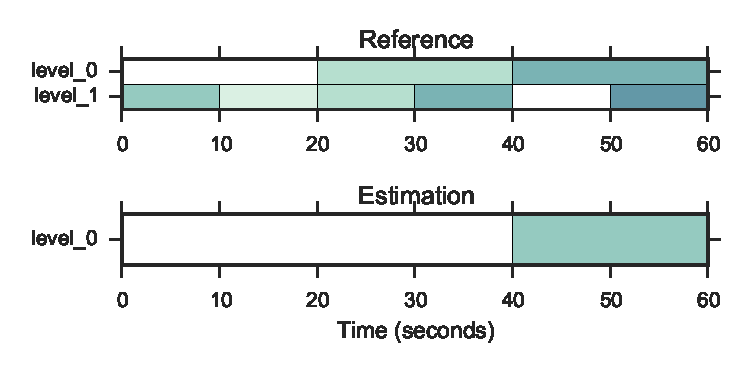
\includegraphics[width=0.94\textwidth]{figs/hier-flatlarger.pdf}
  \end{subfigure}%
  \\
  \begin{minipage}{0.5\textwidth}
    \small
    \centering
    \vspace{10pt}
    \begin{tabular}{l|rr|rr}
      & \multicolumn{2}{c|}{\textbf{Reduced}} & \multicolumn{2}{c}{\textbf{Full}} \\
      $w$       & $\shag_R$    & $\shag_P$  & $\shag_R$ & $\shag_P$    \\
      \hline
      0.5       & 0.0      & 1.00   & 0.20 & 1.00   \\     
      3         & 0.0      & 1.00   & 0.20 & 1.00   \\
      15        & 0.19     & 0.94   & 0.26 & 0.94 \\
      30        & 0.37     & 0.71   & 0.44 & 0.71 \\
      $\infty$  & 0.53     & 0.67     & 0.59 & 0.67\\
    \end{tabular}
  \end{minipage}
  \caption{Hierarchical reference vs.\ flat under-segmentation (top) and $T$-measures
  (bottom).}
  \label{fig:hier-flatlarger}
\end{figure}


\subsubsection{Small-scale and over-segmentation}

% Since, as in the large scale case, we are not over-segmenting, the over-segmentation grades are 100\% for all the time windows.
\Cref{fig:hier-flatsmall} illustrates an example comparable to \Cref{fig:hier-flatlarge}, except that the
estimate now corresponds to the bottom layer of the reference annotation.
Because the reference and estimate agree at the lowest level, every triple derived from
$H_E$ is satisfied in $H_R$, and the precision score is maximal for all time windows.
% As opposed to the previous example, now the lower layer of the reference boundaries match exactly with the estimations, that results into perfect under-segmentation scores for the shorter time windows.
% In this case, the higher the $w$, the lower these under-segmentation grades as expected, since we should not evaluate an algorithm as perfect if it only identifies one layer of the hierarchical boundaries found in the reference.
Note, however, that the reference provides strictly more information than the estimate.  For example, the estimate considers samples at $i=15$ and $j=45$ to be equally irrelevant for a 
query at $q=5$, while the reference indicates a preference for $i=15$.
These effects are only apparent with sufficiently large $w$, \ie, larger than the
smallest segment duration (10s).  This can be easily observed in the $\shag_R$
scores in \Cref{fig:hier-flatsmall}, which decline when the window size grows
large enough to span multiple small segments.

Similarly, \Cref{fig:hier-flatsmaller} illustrates an \emph{over-segmentation}, where the
flat estimation
predicts more boundaries than the deepest layer of the reference.  Again, the tree-recall
scores decay when the window captures multiple short segments.
Unlike the over-segmented example in \Cref{fig:hier-flatlarger}, long-range interactions derived from $H_E$ are mostly satisfied by $H_R$, so $\shag_P$ increases
rather than decreases.

\begin{figure}[t]
  \centering
  \begin{subfigure}{0.5\textwidth}
    \centering
    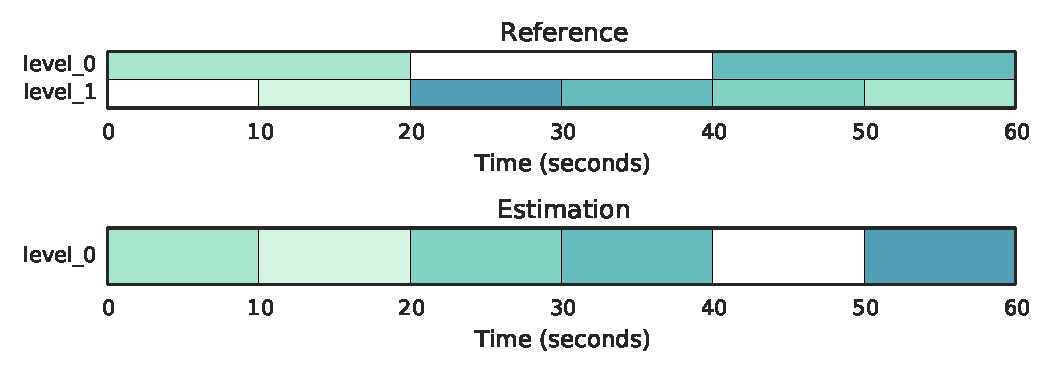
\includegraphics[width=0.94\textwidth]{figs/hier-flatsmall.pdf}
  \end{subfigure}%
  \\
  \begin{minipage}{0.5\textwidth}
    \small
    \centering
    \vspace{10pt}
    \begin{tabular}{l|rr|rr}
      & \multicolumn{2}{c|}{\textbf{Reduced}} & \multicolumn{2}{c}{\textbf{Full}} \\
      $w$       & $\shag_R$    & $\shag_P$  & $\shag_R$ & $\shag_P$    \\
      \hline
      0.5       & 1.00       & 1.00  & 1.00 & 1.00    \\     
      3         & 1.00       & 1.00  & 1.00 & 1.00    \\
      15        & 0.63     & 1.00    & 0.76 & 1.00 \\
      30        & 0.30     & 1.00    & 0.59 & 1.00 \\
      $\infty$  & 0.20     & 1.00   & 0.55 & 1.00
    \end{tabular}
  \end{minipage}
  \caption{Hierarchical reference vs.\ flat, small-scale estimation (top) and $T$-measures (bottom).}
  \label{fig:hier-flatsmall}
\end{figure}

\begin{figure}[t]
  \centering
  \begin{subfigure}{0.5\textwidth}
    \centering
    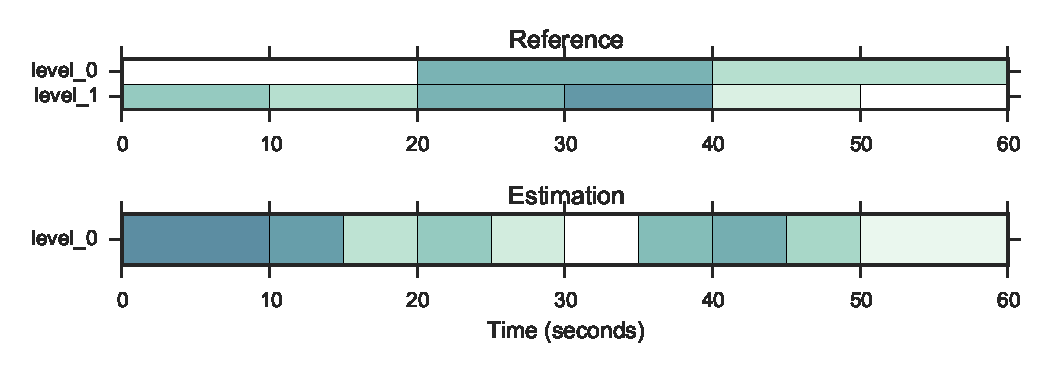
\includegraphics[width=0.94\textwidth]{figs/hier-flatsmaller.pdf}
  \end{subfigure}%
  \\
  \begin{minipage}{0.5\textwidth}
    \small
    \centering
    \vspace{10pt}
    \begin{tabular}{l|rr|rr}
      & \multicolumn{2}{c|}{\textbf{Reduced}} & \multicolumn{2}{c}{\textbf{Full}} \\
      $w$       & $\shag_R$    & $\shag_P$  & $\shag_R$ & $\shag_P$    \\
      \hline
      0.5       & 1.00       & 0.56 & 1.0 & 0.56      \\     
      3         & 0.98     & 0.56   & 0.98 & 0.56   \\
      15        & 0.46     & 0.86   & 0.53 & 0.86 \\
      30        & 0.22     & 0.92   & 0.40 & 0.92 \\
      $\infty$  & 0.13     & 0.94    & 0.37 & 0.94
    \end{tabular}
  \end{minipage}
  \caption{Hierarchical reference vs.\ flat over-segmentation (top) and $T$-measures (bottom).}
  \label{fig:hier-flatsmaller}
\end{figure}
\subsection{Hierarchical vs.\ hierarchical}

% To start with, we demonstrate $T$-measures when comparing two equal hierarchical boundaries in \Cref{fig:hier-hier}.
% As expected, $T$-measures returns 100\% for all the different time windows, showing how we can obtain a perfect score when the reference and 
% estimation are exactly the same across all their layers.

% \begin{figure}[t]
%   \centering
%   \begin{subfigure}{0.5\textwidth}
%     \centering
%     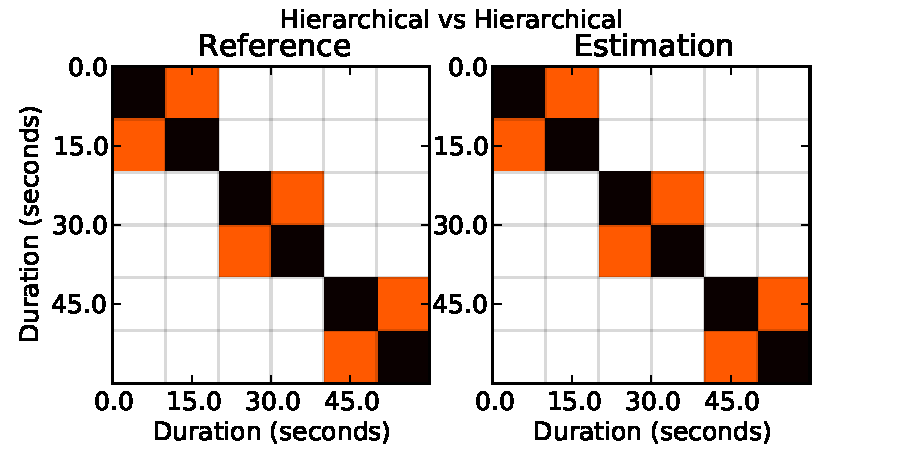
\includegraphics[width=0.94\textwidth]{figs/hier-hier.pdf}
%   \end{subfigure}%
%   \\
%   \begin{minipage}{0.5\textwidth}
%     \centering
%     \vspace{10pt}
%     \begin{tabular}{|c|c|c|}
%       \hline
%       $w$       & $\shag_R$    & $\shag_P$      \\
%       \hline
%       any       & 100       & 100      \\     
%       \hline
%     \end{tabular}
%   \end{minipage}
%   \caption{Hierarchical vs. same hierarchical boundaries (top) and scores (bottom)}
%   \label{fig:hier-hier}
% \end{figure}

In \Cref{fig:hier-hiercomp}, the boundaries (top) and the results (bottom) of two different hierarchical segmentations are shown.
In this case, the estimated boundaries contain a third additional layer covering the first two large segments of its second layer.
Note that the lowest two layers of the estimation are exactly the same as the two layers of the reference.
The scores at small $w$ show a perfect agreement for both $T$-measures, since the window
is not large enough to resolve the differences between reference and estimation.
However, as $w$ increases, we see how the precision score $\shag_P$ decreases as expected, since the
estimation has found an additional segment not captured in the reference.
% (even if this new segment creates a new layer it still oversegments).
The tree-recall scores remain at 100\% for all $w$, as expected.


\begin{figure}[t]
  \centering
  \begin{subfigure}{0.5\textwidth}
    \centering
    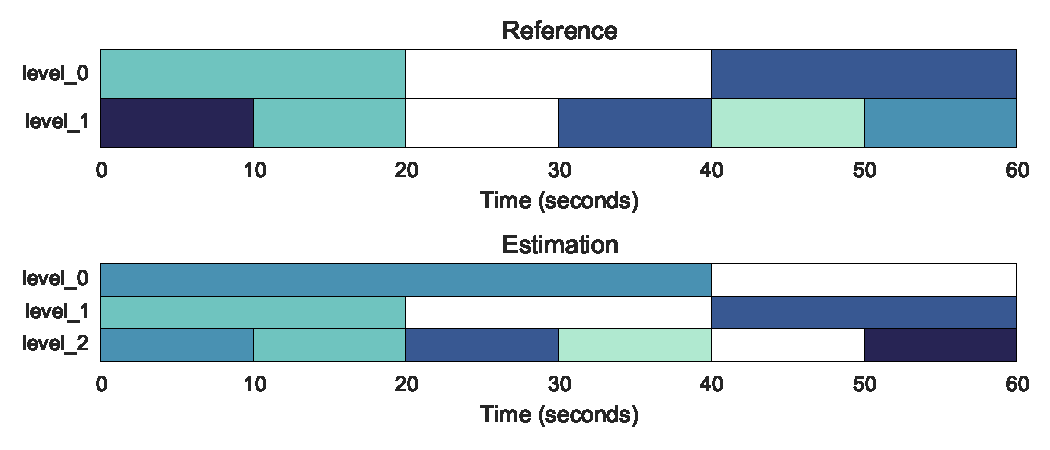
\includegraphics[width=0.94\textwidth]{figs/hier-hiercomp.pdf}
  \end{subfigure}%
  \\
  \begin{minipage}{0.5\textwidth}
    \small
    \centering
    \vspace{10pt}
    \begin{tabular}{l|rr|rr}
      & \multicolumn{2}{c|}{\textbf{Reduced}} & \multicolumn{2}{c}{\textbf{Full}} \\
      $w$       & $\shag_R$    & $\shag_P$  & $\shag_R$ & $\shag_P$    \\
      \hline
      0.5       & 1.00       & 1.00      & 1.00 & 1.00\\     
      3         & 1.00       & 1.00      & 1.00 & 1.00\\
      15        & 1.00       & 0.98      & 1.00 & 0.99\\
      30        & 1.00       & 0.79      & 1.00 & 0.89\\
      $\infty$  & 1.00       & 0.62     & 1.00 & 0.79  
    \end{tabular}
  \end{minipage}
  \caption{2-layer vs. 3-layer hierarchical boundaries (top) and $T$-measures scores (bottom).}
  \label{fig:hier-hiercomp}
\end{figure}


\subsection{Human annotator agreement}
\Cref{fig:SALAMI-SALAMI} illustrates hierarchical annotations obtained from two human annotators on one track in
the SALAMI dataset, using the large- and small-scale segmentations.
While the two annotators tend to agree at the small scale, they differ at the large scale.
This is reflected in the $T$-measures: at large $w$, the recall skews low because the 
reference's large-scale annotations are coarser than those of the estimation, while the precision remains high because both tend to agree at the small scale.

\begin{figure}[t]
  \centering
  \begin{subfigure}{0.5\textwidth}
    \centering
    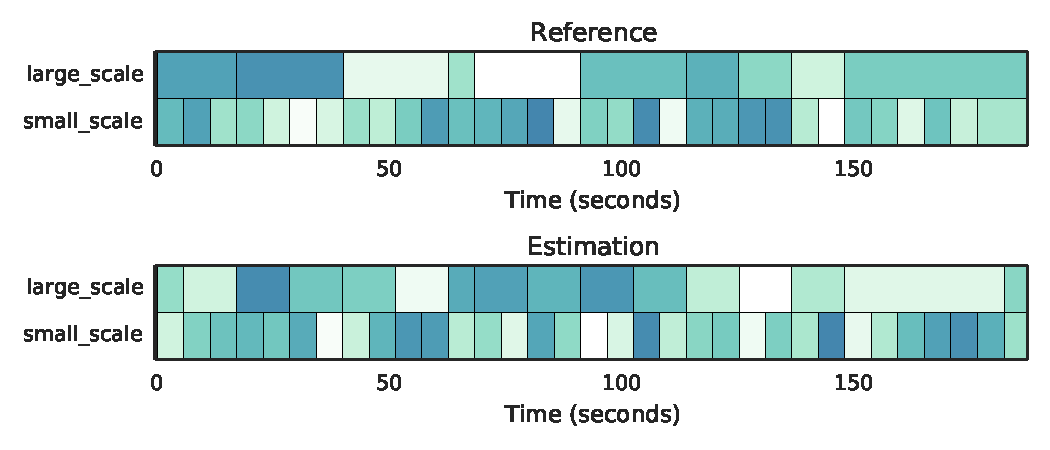
\includegraphics[width=0.99\textwidth]{figs/SALAMI-SALAMI.pdf}
  \end{subfigure}%
  \\
  \begin{minipage}{0.5\textwidth}
    \small
    \centering
    \vspace{10pt}
    \begin{tabular}{l|rr|rr}
      & \multicolumn{2}{c|}{\textbf{Reduced}} & \multicolumn{2}{c}{\textbf{Full}} \\
      $w$       & $\shag_R$    & $\shag_P$  & $\shag_R$ & $\shag_P$    \\
      \hline
      0.5       & 0.76       & 0.77      & 0.81 & 0.79\\     
      3         & 0.95       & 0.95      & 0.96 & 0.93\\
      15        & 0.75       & 0.75     & 0.80 & 0.84\\
      30        & 0.62       & 0.83     & 0.71 & 0.89\\
      $\infty$  & 0.57       & 0.96 & 0.68 & 0.98
    \end{tabular}
  \end{minipage}
  \caption{Hierarchical annotations for SALAMI track \#636 from the two different human
  annotators. Top: annotations; bottom: $T$-measures scores.}
  \label{fig:SALAMI-SALAMI}
\end{figure}

\begin{figure}
    \centering
    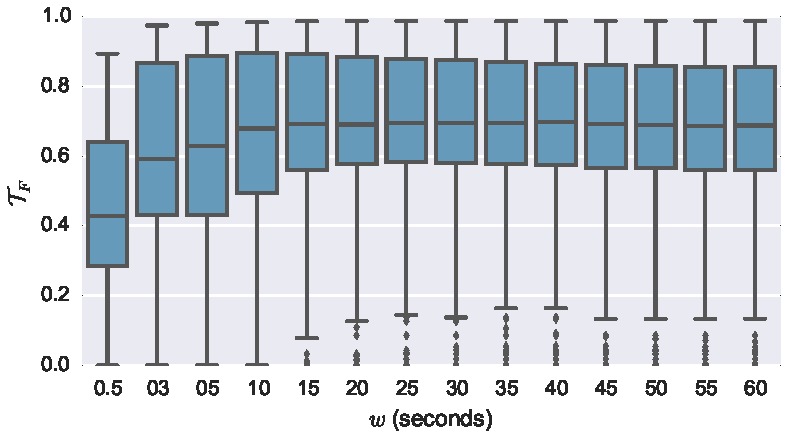
\includegraphics[width=\columnwidth]{figs/tfw}
    \caption{$\shag_F$ scores between human annotators for SALAMI tracks over a range of window sizes $w$.\label{fig:salami-agree}}
\end{figure}

To further investigate inter-annotator agreement, we computed $T$-measure scores between hierarchical
reference annotations for 410 tracks in the SALAMI dataset.  To simplify the analysis, we
summarize agreement by $\shag_F$. \Cref{fig:salami-agree} illustrates the distribution of
per-track $\shag_F$ scores as a function of $w$.  We observe that the score distribution is relatively stable
for $w \geq 15$.\footnote{The analogous plots for $\shag_P$ and $\shag_R$ are omitted for brevity, but illustrate the same
trend.} 
The example given in \Cref{fig:SALAMI-SALAMI} lies slightly above the average agreement
($\shag_F = 0.75$ at $w=15$),
but is generally representative of inter-annotator agreement.
The out-lying low scores tend to be examples where one annotator simply ignored structure annotated
by the other: for example, one annotator only marked \emph{silence} boundaries in track \#68.

This analysis reemphasizes prior observations that humans do not perfectly agree upon structural
annotations~\cite{Smith2013}, and suggests an accuracy ceiling near 70\% for hierarchical boundary detection.
Similarly, it suggests that $w=15$ provides a reasonable default value for the SALAMI dataset.  This setting
is large enough to capture multiple small-scale segments: in the tracks considered for this evaluation, 
the median small-scale segment duration was 6.66s, with a 95th percentile of 15.69s.

% SALAMI 636 annotator 1 vs. OLDA\cite{McFee2014}  output \ref{fig:SALAMI-OLDA}.
\subsection{Annotator vs.\ algorithm}
Finally, \Cref{fig:SALAMI-OLDA} compares a hierarchical estimation against a hierarchical reference.
The hierarchical estimation was produced by the agglomerative clustering method of McFee and Ellis~\cite{McFee2014}.
Note that the estimate produces many more layers than the reference, and the nesting
structure is quite different, since each layer introduces only a single new segment.
The reference provides only two levels of segmentation (large and small), while the 
estimate produces mainly large segments, but exposes more structure among them.
Consequently, the scores are lower than the annotator-agreement scores listed in
\Cref{fig:SALAMI-SALAMI}.

\begin{figure}[t]
  \centering
  \begin{subfigure}{0.5\textwidth}
    \centering
    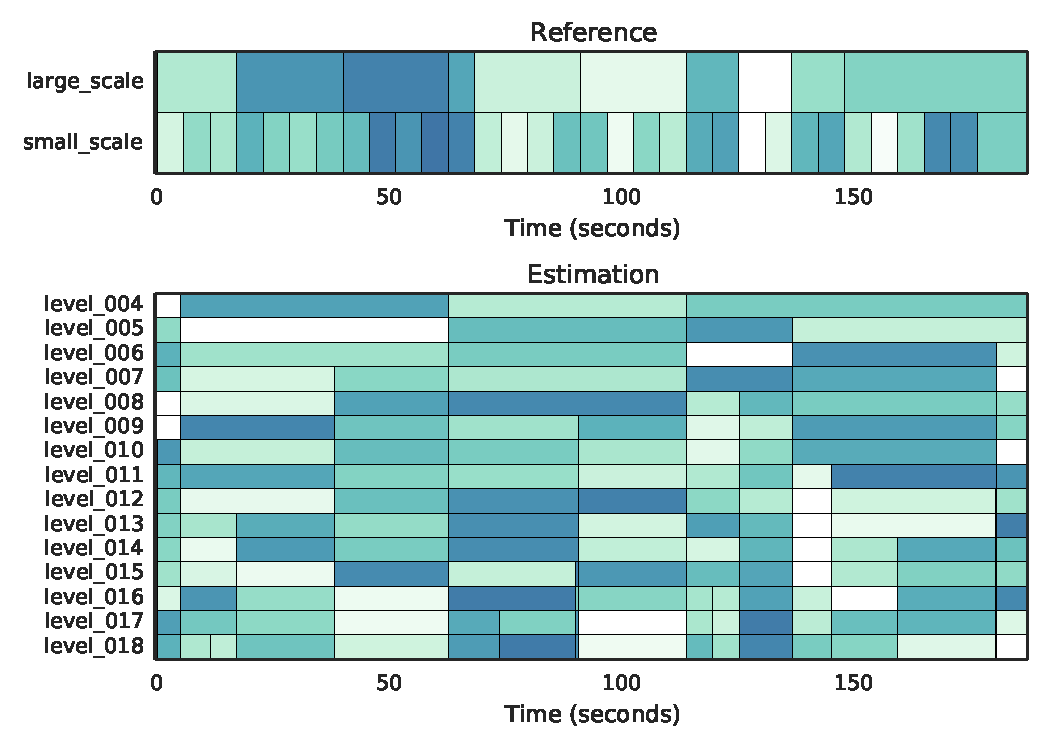
\includegraphics[width=0.94\textwidth]{figs/SALAMI-OLDA.pdf}
  \end{subfigure}%
  \\
  \begin{minipage}{0.5\textwidth}
    \small
    \centering
    \vspace{10pt}
    \begin{tabular}{l|rr|rr}
      & \multicolumn{2}{c|}{\textbf{Reduced}} & \multicolumn{2}{c}{\textbf{Full}} \\
      $w$       & $\shag_R$    & $\shag_P$  & $\shag_R$ & $\shag_P$    \\
      \hline
      0.5       & 0.14       & 1.00  & 0.28 & 0.55 \\
      3         & 0.20       & 1.00  & 0.34 & 0.72    \\
      15        & 0.62       & 0.56  & 0.66 & 0.70 \\
      30        & 0.76       & 0.53  & 0.80 & 0.58  \\
      $\infty$  & 0.90       & 0.16  & 0.93 & 0.42
  \end{tabular}
  \end{minipage}
  \caption{Hierarchical annotation for SALAMI track \#636 vs.\ hierarchical boundary
  estimates~\cite{McFee2014} (top) and $T$-measures scores (bottom).}
  \label{fig:SALAMI-OLDA}
\end{figure}

%\section{Evaluating Automatic Algorithm}

%Olda\cite{McFee2014} with SALAMI.


\section{Discussion}\label{sec:conclusions}

The implementation of $T$-measures depends upon two critical parameters: the time window
$w$, and whether to use the \emph{reduced} or \emph{full} metrics.  While the setting of
$w$ ultimately depends upon the practitioner's preference and characteristics of the
dataset, the results on SALAMI suggest that $w=15$ provides a reasonable balance
between capturing high-level structure and resilience to long-range interactions.
As illustrated in \cref{sec:largeover}, when $w$ is large enough to capture multiple short
segments, the transitive reduction approach can also be used to enhance the range
of the metric while eliminating redundant comparisons.

In this paper, we focused only on the problem of evaluating estimated boundaries.
In future work, we plan to extend general ideas behind $T$-measures to other structural 
annotation problems, such as segment label agreement.

\bibliography{refs}

\end{document}
